\documentclass{article}
\usepackage{a4}
\usepackage{amsmath}
\usepackage{amsthm}
\usepackage{amssymb}
\usepackage{indentfirst}
\usepackage{verbatimbox,hyperref}
\usepackage[T1]{fontenc}
\usepackage[utf8]{inputenc}
\usepackage{tikz}
\usetikzlibrary{matrix}
\def\leftbracket{[}
\def\rightbracket{]}
\usepackage{tikz}

\usetikzlibrary{shapes,arrows,calc}
\newcommand{\data}{data \nodepart{second} \phantom{null}}
\usetikzlibrary{matrix,positioning,arrows.meta,arrows}
\usepackage{graphicx}
\usepackage{subcaption}

\tikzstyle{ptr}  = [draw, -latex']
\tikzstyle{head} = [rectangle, draw, text height=3mm, text width=3mm, text centered, node distance=3cm, inner sep=0pt]
\tikzstyle{data} = [rectangle split, rectangle split parts=2, draw, text centered, minimum height=3em]


\title{Graph Storage: How good is CSR really?}
\author{Mahammad Valiyev}

\begin{document}
\maketitle

\begin{abstract}
  In the last decade, the data size is growing exponentially and processing those data is becoming a difficult problem. Nowadays researchers and industry have been interested in the analysis of the graph to get deep understanding of social networks. Many of these graphs used in industry have become very large, containing hundreds of millions of nodes and edges. In this paper, I propose Compressed Sparse Row(CSR) which is a fast graph container. My CSR implementation also supports updates on graph. On a static graph, CSR gives ~ up to 3x better performance over Adjacency List Implementation(AL) on Depth-First-Search(DFS) and Breadth-First-Search(BFS) and sometimes better performance on Dijkstra algorithm(Shortest path).
\end{abstract}
\textbf{Keywords:} Graph databases, Compressed Sparse Row

\section{Introduction}
Graph analysis have become more popular in the last few years. Graphs are usually used to represent social networks in which vertices indicate users and edges indicate friendship between users. Facebook has 1.39 billion  active users as of 12/2014 with more than 400 billion edges\cite{fb}. Therefore, processing big graphs is consuming more time as the number of users and relationships significantly increased. The proposed approach(CSR) gives slightly better performance over the other approach on DFS algorithm. BFS algorithm in general is faster than DFS as it doesn't have an additional overhead of recursion. CSR gives a bit much better on BFS. In the following subsections, I will give some details about CSR and two variants of AL. In the following, I will give some details about existing approaches in Section 2, then followed by implementation details(Section 3) and an evaluation(Section 4). In Section 5 I will give conclusion about how good CSR is really.

\section{Related Works}
STINGER\cite{stinger} is a mutable graph container which is capable of handling updates which can be inserted parallel. it uses a fixed-size chained buckets to keep edges. Due to its loosely synchronized parallel updates that only maintains physical consistency of the data structure, a query may see the graph in a state that never existed. Each bucket contains only edges of the same type.\\
LLAMA\cite{llama} is a new extention to CSR with the support of versioning. It provides consistent snapshots on the graph and allow multiple accesses to them. At first, updates are buffered in a change set and after some period of time creates a new snapshots with the updates on change set. The main drawback is that the method usually has many existing snapshots and accessing to the newer snapshots consume more time. it merges old snapshots and apply a delta to CSR. \\
ASGraph\cite{asgraph} is also a new extention to which reduce update time to very small latency by breaking up the edge list of CSR into multiple chunks and that support efficient mutation and employing an append-only scheme for updates.
 
\section{Implementation}
 I have implemented a nice graph interface for CSR graph container and two variants of AL in which graph algorithms can easily be built upon on that. Thus, graph algorithms are independent of the type of graph container. Moreover, modifications on graph containers don't affect the algorithms. For the future work, new algorithms can easily be implemented using the methods of graph containers. In the following subsections, I will briefly explain all three graph containers and show how the edges are actually stored in the memory for sample graph in Figure 1.
\begin{center} 
 
 \begin {tikzpicture}[-latex ,node distance =3 cm and 3cm ,on grid ,
semithick ,
state/.style ={ circle, draw  , minimum width =1 cm}]
\node[state] (A) {$1$};
\node[state] (B) [below=of A] {$2$};
\node[state] (C) [right =of A] {$3$};
\node[state] (D) [below =of C] {$4$};

\path (A) edge [bend right = 25] node[right] {} (B);
\path (A) edge [bend left = 25] node[right] {} (C);
\path (A) edge  node[right] {} (D);
\path (C) edge [bend left = 25] node[right] {} (D);
\path (C) edge [bend left = 25] node[right] {} (A);
\path (B) edge [bend right = 25] node[right] {} (D);
\path (D) edge [bend right = 25] node[right] {} (B);
\path (D) edge [bend left = 25] node[right] {} (C);


\node[align=center, yshift=-1em] (title) 
    at (current bounding box.south)
    {\textbf{Figure 1:} Small sample graph with four nodes};
\end{tikzpicture}
\end{center}

\subsection{Compressed Sparse Row}
In CSR format, all edges are stored in the same array called \texttt{edges} and an addditional \texttt{offsets} array is used to get the first neighbor of a node. For each node, the number of neighbors for a node \texttt{n} can be calculated \texttt{offsets[n+1]-offsets[n]}. Figure 1 shows a small graph with four nodes with few edges and Figure 2 shows the corresponding CSR.\\

\tikzset{
mymat/.style={
  matrix of math nodes,
  text height=2.5ex,
  text depth=0.75ex,
  text width=3.25ex,
  align=center,
  column sep=-\pgflinewidth
  },
mymats/.style={
  mymat,
  nodes={draw,fill=#1}
  }  
}



\begin{center}

\begin{tikzpicture}[>=latex]
\matrix[mymat,anchor=west,row 2/.style={nodes=draw}]
at (1,1) 
(mat1)
{
0 & 1 & 2 & 3 & 4 & 5 & 6 & 7 & \\
1 & 2 & 3 & 4 & 1 & 4 & 2 & 3 & \\
};
\matrix[mymat,below=of mat1,row 2/.style={nodes=draw}]
at (4,0.7)
(mat2)
{
  &   &   &  &  \\
0 & 3 & 4 & 6 & 8\\
};



\begin{scope}[shorten <= -2pt]
\draw[*->]
  (mat2-2-1.north)  --  (mat1-2-1.south west);
\draw[*->]
  (mat2-2-2.north)  --  (mat1-2-4.south west);
\draw[*->]
  (mat2-2-3.north)  --  (mat1-2-5.south west);
\draw[*->]
  (mat2-2-4.north)  --  (mat1-2-7.south west);
\draw[*->]
  (mat2-2-5.north)  --  (mat1-2-8.south east);
    
\end{scope}

\matrix[mymat,below=of mat1,row 2/.style={nodes=draw}, below of=mat2]
at (4,0.57)
(mat3)
{
1  & 2 & 3 & 4 & - \\
 &  &  &  & \\
};

\node[] at (0.4,0.63)
  (cella) {\texttt{edges}};

\node[] at (1.2,-0.82)
  (cellb) {\texttt{offsets}};

\node[xshift=-1.35em, yshift=0em] (title) 
    at (mat3.south)
    {\textbf{Figure 2:} CSR format of the sample graph};

\end{tikzpicture}
\end{center}

All edges are kept densely in the main memory. While iterating over all neighbors of all nodes, the common task in graph algorithms is mostly memory accesses which are usually sequential accesses. As it is a sequential access, the accesses to \texttt{edges} and \texttt{offsets} arrays are also sequential. It is indeed a beneficial memory access pattern as CPU can easily predict and prefetch. Therefore most of the memory accesses hit the cache. In case of non-sequential access, CSR is not cache-friendly.

\subsection{Ajdacency List with \texttt{std::list}}
In this format, all edges which are outgoing are stored in \texttt{std::list}, thus at the beginning for each node a \texttt{std::list} is kept. According to the structure of \texttt{std::list}, the elements of \texttt{std::list} are not located sequentially in the memory. Moreover, it is not cache-friendly at all. \\

\begin{center}
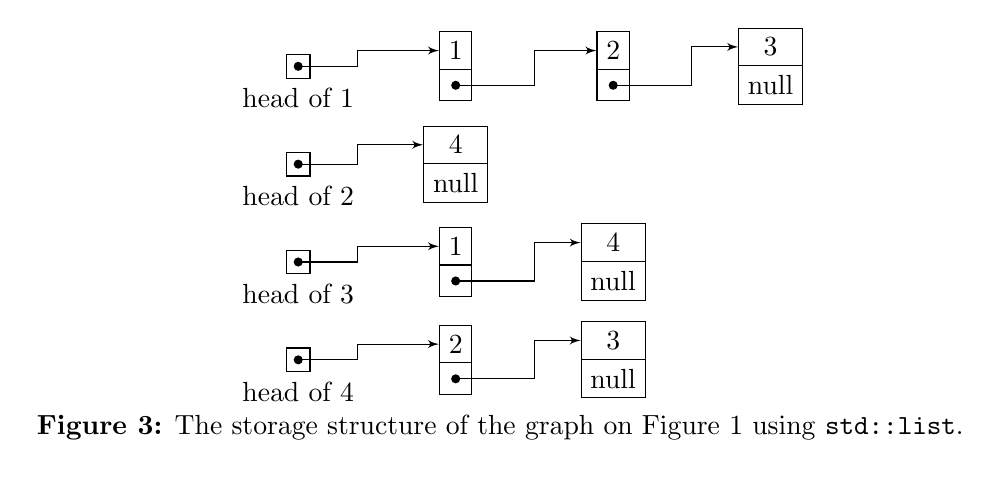
\begin{tikzpicture}[node distance=2cm, auto]

    \node[head, label=below:head of 1] (head1) {};
    \node[data, right of=head1]    (A1) {1};
    \node[data, right of=A1]       (B1) {2};
    \node[data, right of=B1]       (C1) {3 \nodepart{second} null};

    \draw[fill] (head1.center)   circle (0.05);

    \path[ptr]  (head1.center) --++(right:7.5mm)  |- (A1.text west);
    \draw[fill] ($(A1.south)!0.5!(A1.text split)$) circle (0.05);
    \draw[ptr]  ($(A1.south)!0.5!(A1.text split)$) --++(right:10mm) |- (B1.text west);
    \draw[fill] ($(B1.south)!0.5!(B1.text split)$) circle (0.05);
    \draw[ptr]  ($(B1.south)!0.5!(B1.text split)$) --++(right:10mm) |- (C1.text west);
    
    
    \node[head, label=below:head of 2, below of=head1, yshift=5em] (head2) {};
    \node[data, right of=head2]    (A2) {4 \nodepart{second} null};    
    \draw[fill] (head2.center)   circle (0.05);
    \path[ptr]  (head2.center) --++(right:7.5mm)  |- (A2.text west);

	
	\node[head, label=below:head of 3, below of=head2, yshift=5em] (head3) {};
    \node[data, right of=head3]    (A3) {1};
    \node[data, right of=A3]       (C3) {4 \nodepart{second} null};

    \draw[fill] (head3.center)   circle (0.05);

    \path[ptr]  (head3.center) --++(right:7.5mm)  |- (A3.text west);
    \draw[fill] ($(A3.south)!0.5!(A3.text split)$) circle (0.05);
    \draw[ptr]  ($(A3.south)!0.5!(A3.text split)$) --++(right:10mm) |- (C3.text west);
    
    \node[head, label=below:head of 4, below of=head3, yshift=5em] (head4) {};
    \node[data, right of=head4]    (A4) {2};
    \node[data, right of=A4]       (C4) {3 \nodepart{second} null};

    \draw[fill] (head4.center)   circle (0.05);

    \path[ptr]  (head4.center) --++(right:7.5mm)  |- (A4.text west);
    \draw[fill] ($(A4.south)!0.5!(A4.text split)$) circle (0.05);
    \draw[ptr]  ($(A4.south)!0.5!(A4.text split)$) --++(right:10mm) |- (C4.text west);
	\node[xshift=5.3em, yshift=-2em, xshift=2em] (title) 
    at (head4.south)
    {\textbf{Figure 3:} The storage structure of the graph on Figure 1 using \texttt{std::list}.};

\end{tikzpicture}
\end{center}

As shown from Figure 3, \texttt{std::list} doesn't show any cache friendly structure. Thus, usage of it only gives us better update latency.

\subsection{Ajdacency List with \texttt{std::vector}}
Second approach of Adjacency List uses \texttt{std::vector} structure to keep outgoing edges for each node. \texttt{std::vector} also uses an array structure to keep the elements, however whenever it hits the capacity, it creates new doubled size array and copies the contents of the old one including the newly added element, then removes the old one. It may seem to be like a big overhead, but in reality it only does \texttt{3*n} additional operations for \texttt{n} inserts into it. \\

\tikzset{
mymat/.style={
  matrix of math nodes,
  text height=2.5ex,
  text depth=0.75ex,
  text width=3.25ex,
  align=center,
  column sep=-\pgflinewidth
  },
mymats/.style={
  mymat,
  nodes={draw,fill=#1}
  }  
}



\begin{center}

\begin{tikzpicture}[>=latex]
\matrix[mymat,anchor=west,row 2/.style={nodes=draw}]
at (1,1) 
(mat1)
{
 &  &  & \\
1 & 2 & 3 & \phantom{x}\\
};
\node[] at (0.15,0.93)
  (cella) {\texttt{edges[1]}};

\matrix[mymat,anchor=west,row 2/.style={nodes=draw}, below of=mat1]
at (1.5,1) 
(mat2)
{
 \\
4 \\
};
\node[] at (0.15,0)
  (cellb) {\texttt{edges[2]}};

\matrix[mymat,anchor=west,row 2/.style={nodes=draw}, below of=mat2]
at (1.88,0) 
(mat3)
{
 &   \\
1 & 4 \\
};
\node[] at (0.15,-1)
  (cellc) {\texttt{edges[3]}};

\matrix[mymat,anchor=west,row 2/.style={nodes=draw}, , below of=mat3]
at (1.88,-1) 
(mat4)
{
 &  \\
2 & 3 \\
};
\node[] at (0.15,-2)
  (celld) {\texttt{edges[4]}};



\node[xshift=5.3em, yshift=-1.3em] (title) 
    at (celld.south)
    {\textbf{Figure 4:} The storage structure of the graph on Figure 1 using \texttt{std::vector}.};

\end{tikzpicture}
\end{center}

As it is shown in Figure 4, \texttt{std::vector} implementation also has a cache-fiendly structure.

\section{Evaluation}
All three approches are tested on different datasets which are generated randomly. The number of users is 1,000,000. To make it as a real social network, the number of neighbors differs from 50 to 200. In the following subsections, I discuss in which scenario CSR gives better performance in terms of latency and memory consumption. My test machine is a single socket server computer equipped with Intel(R) Core(TM) i7-3930K CPU 6-core @ 3.20GHz and 64 GB of main memory. This server has 12 hardware cores (with hyperthreading enabled).

\subsection{Algorithm comparisons}
To get a feeling of how fast CSR is compared to Adjacency list, I evaluate three different widely used and simple algorithms that cover a wide-ranging graph access patterns.
\subsubsection*{Depth-first search and Breadth-first search}
DFS is a mainly read-only graph search algorithm which usually reads them sequentially. However on BFS, it also read and write to an additional queue. Theoretically both algorithms should be \textit{O(n)}. However depending on the depth of tree for DFS and the size of queue for BFS, one of the algorithms may perform better than the other one. In the following section, due to the property of sequential read, CSR performs better than Ajdacency List.
\begin{figure}[h]
\begin{subfigure}[h]{0.49\textwidth}
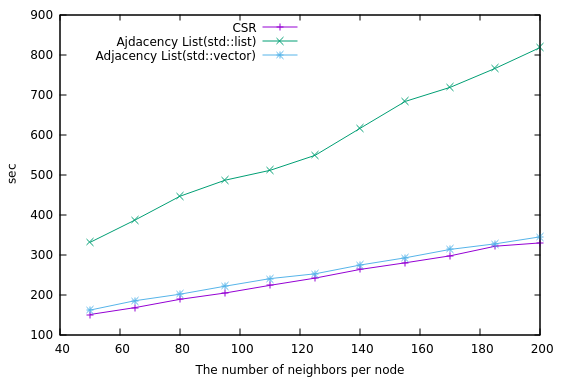
\includegraphics[scale = 0.425]{DFS}
\caption{Result for DFS}\label{fig:figA}
\end{subfigure}
\begin{subfigure}[h]{0.49\textwidth}
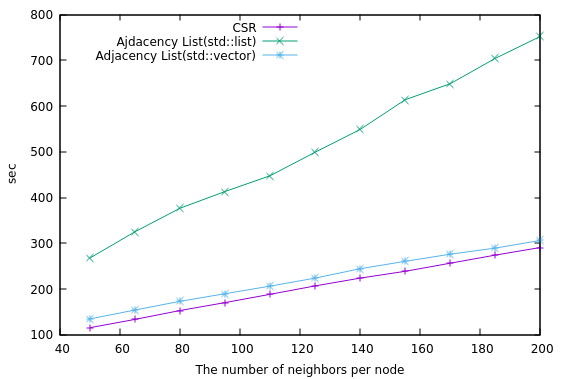
\includegraphics[scale = 0.425]{BFS}
\caption{Result for BFS}\label{fig:figB}
\end{subfigure}
\caption*{\textbf{Figure 5}: Results of DFS and BFS for the graph with 1,000,000 nodes.}
\end{figure} \\
 I test the system with 200 DFS and BFS in which it starts from a random node. CSR is up to 3 times faster than \texttt{std::list} approach. For \texttt{std::vector}, CSR finishes it at least 15 secs earlier.

\subsubsection*{Dijkstra Algorithm}
Dijkstra algorithm solves the shortest path problem between two nodes in the graph. The complexity of the algorithm is \textit{O(nlogn)}. Despite the fact that it heavily reads the data from main memory, the most time consuming operation is insertion into priority queue which takes \textit{O(logn)}. Thus in the evaluation of Dijkstra, it is difficult to interpret anything from the result.\\
\begin{center}
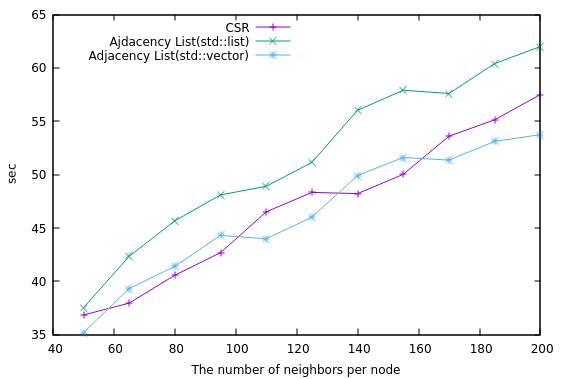
\includegraphics[scale = 0.6]{Dijkstra}\\
\textbf{Figure 6}: Results of Dijkstra for the graph with 1,000,000 nodes.
\end{center}
 CSR is still better on Dijkstra algorithm than \texttt{std::list} approach. It is difficult to say whether CSR or \texttt{std::vector} is better than the other one.
\subsection{Complex Scenario}
 I have implemented two different update structures for CSR. As it is seen from the structure of Adjacency List on Section 3, updates on Adjacency List is super fast operation which just appends the newly added edge to the corresponding list. It takes much less than a milli second. For CSR, it is too heavy operation to handle. In the following subsection, I will explain how both update structures works and how fast they are.
 
 \subsubsection*{Simple Update}
   Assume that the directed graph has \textit{V} nodes and \textit{E} edges. To keep the structure of CSR, we need to allocate a new array with \textit{E}+\textit{1} edges for each newly added edge. Let's call the new array as \texttt{edges'} and the new edge is \textit{e=(v,u)}. First of all, I copy all the content of the array \texttt{edges} from \texttt{offsets[1]} to \texttt{offsets[v+1]} and the rest content of the array \texttt{edges} to the array \texttt{edges'} starting from \texttt{offsets[v+1] + 1} index. Then I set \texttt{edges'[offsets[v+1]]=u}. At the end, I increment all the elements from \texttt{offsets[v+1]} to \texttt{offsets[V+1]}. To copy the content of array, I use \texttt{std::memcpy} function which is better than \texttt{std::memmove} function. 
 \subsubsection*{Light Update}
 As it is shown from the results of \textbf{\textit{Simple Update}}, it is the most time consuming operation for CSR format. A new update structure -\textbf{\textit{Light Update}}- is a much faster update method compared to \textbf{\textit{Simple Update}}.\\
 The new approach is built on top of the previous approach. As an addition, the structure of CSR format should be modified in this method. Assume that we are given a directed graph which has \textit{V} nodes and \textit{E} edges. \texttt{edges} array should have more than |\textit{E}|, which I call it as \textit{additional space}. For each new upcoming edge, CSR doesn't need to allocate a new big \texttt{edges} array to store a new one. Let's call the new edge as \textit{e=(v,u)}. It does a new allocation whenever \texttt{edges} array hits the capacity. If it is already full, the update is exactly the same as in \textbf{\textit{Simple Update}}. If the \texttt{edges} array still has some space to store new edges, I copy all the array elements from \texttt{offsets[v+1]} into \texttt{edges} array starting from \texttt{offsets[v+1] + 1} index. As there is intersection between source and destination, I use \texttt{std::memmove} function to do this copy operation. Then I set the corresponding element to \texttt{u} and increment corresponding elements of \texttt{offsets} array as it is in \textbf{\textit{Simple Update}}. As it is shown, CSR doesn't do new allocation and copy all the array for each update. The speed-up comes along with having very few new allocations and copying.\\
\begin{center}
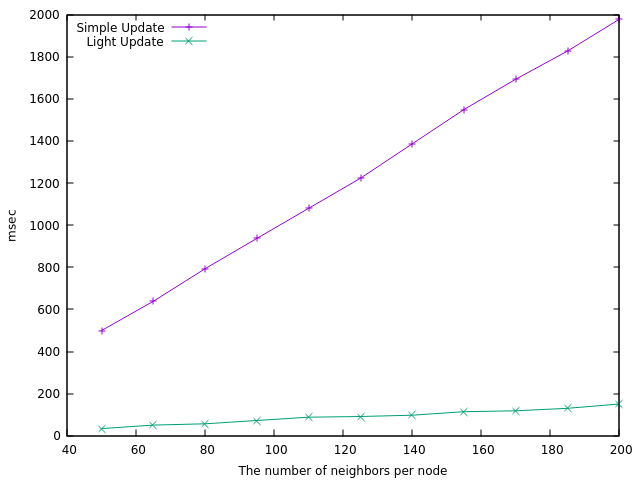
\includegraphics[scale = 0.5]{time_per_update}\\
\textbf{Figure 7}: Latencies of both updates for the graph with 1,000,000 nodes.
\end{center}

 As it is shown from Figure 7, \textbf{\textit{Light Update}} always performs ~13-15x faster than \textbf{\textit{Simple Update}}. This gives us a possibility to use CSR for temporal graphs as well.
 
 \subsubsection*{Real World Example}
 I evaulate the system in a mixed workload in which every 20th operation of queries is an update query(\textbf{\textit{Light Update}}) which adds a new edge to the graph. Therefore, it gives us an overview of how good CSR is really on temporal graphs.
 \begin{center}
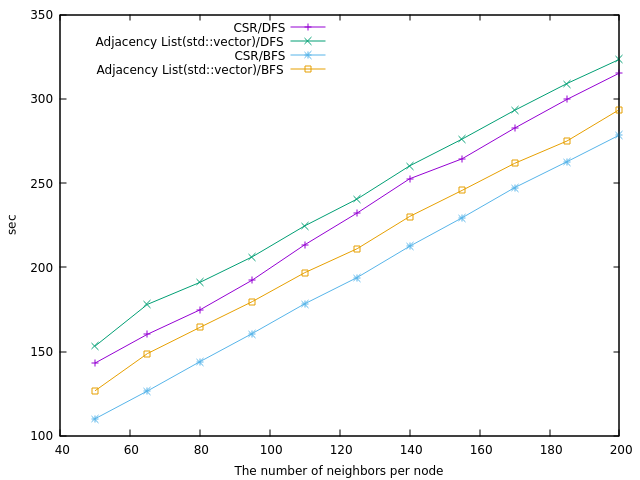
\includegraphics[scale = 0.5]{mixed_workload}\\
\textbf{Figure 8}: Latencies for mixed workload for the graph with 1,000,000 nodes.
\end{center}
 Figure 8 shows that CSR is still performing better in the case of having every 20th operation as update. Thus, CSR can be an option for temporal graphs. However, \textbf{\textit{Light Update}} is too heavy operation for much bigger graphs. Further investigation should be done on bigger graphs.
 
\subsubsection*{An Interesting Approach to Real World Example} 
 Real-world graphs are usually clustered. Therefore, the likelihood that a neighbor is already in the cache is higher if you access them in a sorted manner. One might label nodes in such a way that neighbors have similar ids. I have generated a graph with 1,000,000 nodes in which each node has neighbors between 50 and 200 and all neighbors have similar ids. 
 \begin{figure}[h]
\begin{subfigure}[h]{0.5\textwidth}
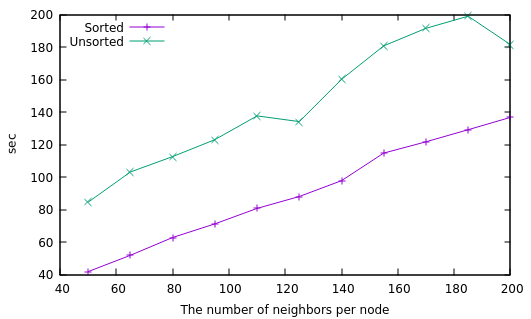
\includegraphics[scale = 0.45]{DFS_sorted}
\caption{Result for DFS}\label{fig:figA}
\end{subfigure}
\begin{subfigure}[h]{0.6\textwidth}
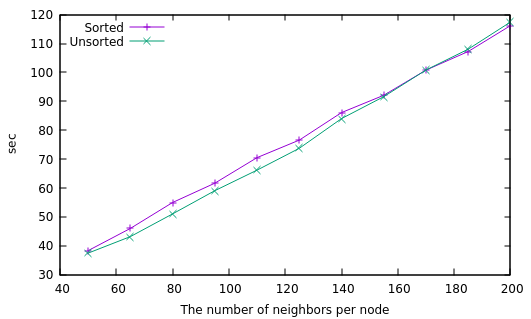
\includegraphics[scale = 0.45]{BFS_sorted}
\caption{Result for BFS}\label{fig:figB}
\end{subfigure}
\caption*{\textbf{Figure 9}: Results of DFS and BFS for the graph stores neighbors in sorted.}
\end{figure} \\
 For DFS, keeping neighbors in sorted way gives us 1.6-2.1x less latency. However, for BFS it doesn't really decrease the time. One can interpret from here that it is always better to keep neighbors sorted in CSR. In order to keep sorted structure, additional overhead is just to do binary search to find the corresponding index for new edge which is just \textit{O(logn)}. 
 
\subsection{Memory consumption}
  So far we only compared CSR with other two approaches in terms of latency. For the real world use, memory consumption should be considered as one of the main property. 



\begin{center}
\begin{tabular}{ |p{2cm}||p{4cm}|p{4.5cm}|}
 \hline
\# neighrbors per node & mem(std:list)$\div$mem(CSR) & mem(std:vector)$\div$mem(CSR)\\
 \hline
 50   & 7.33&1.41\\
 65&   7.46  & 2.01  \\
 80 &7.55 & 1.66\\
 95    &7.62 & 1.42\\
 110&   7.67  & 1.23\\
 125& 7.7  & 1.15 \\
 140& 7.73  & 1.85\\
 155& 7.76  & 1.68\\
 170& 7.78  & 1.54\\
 185& 7.79  & 1.42\\
 200& 7.81  & 1.31\\
 \hline
\end{tabular}\\
\textbf{Table 1}: Ratio of memory consumption of CSR with other approaches.
\end{center}



\texttt{std::list} is usually implemented as doubly linked list. Because of this structure it uses much more memory. But according to the structure of \texttt{std::vector}, each of them is at least half full for each node, whereas there are some empty places. However CSR has only one memory overhead which is \texttt{offsets} array. As shown from Table 1, CSR is always using less memory than the other approaches, at least 7 times less than \texttt{std::list} and around 1.15 times less than \texttt{std::vector}.

\section{Conclusion}
As it is shown from the results, CSR is not that superior to other two approaches. But considering the fact that social networks are growing so fast nowadays, a slight better approach significantly matters. While most analysis still focuses on static graphs, in the future there will be huge demand on temporal graphs. As CSR itself is not update-friendly, more investigation should be done on the variants of CSR. The CSR library, together with two Adjacency List implementation and generation of graphs, is available online at \texttt{https://github.com/mehemmedv/DB\_Imp\_Seminar}\\

\begin{thebibliography}{}
\bibitem{fb}
Ching, A., Edunov, S., Kabiljo, M., Logothetis, D., \and Muthukrishnan, S. (2015). One trillion edges: Graph processing at facebook-scale. Proceedings of the VLDB Endowment, 8(12), 1804-1815
\bibitem{stinger}
Ediger, D., McColl, R., Riedy, J., \and Bader, D. A. (2012, September). Stinger: High performance data structure for streaming graphs. In High Performance Extreme Computing (HPEC), 2012 IEEE Conference on (pp. 1-5). IEEE.
\bibitem{llama}
Macko, Peter, Virendra J. Marathe, Daniel W. Margo, and Margo I. Seltzer. "LLAMA: Efficient graph analytics using large multiversioned arrays." In Data Engineering (ICDE), 2015 IEEE 31st International Conference on, pp. 363-374. IEEE, 2015.
\bibitem{asgraph}
Haubenschild, Michael, Manuel Then, Sungpack Hong, and Hassan Chafi. "ASGraph: a mutable multi-versioned graph container with high analytical performance." In Proceedings of the Fourth International Workshop on Graph Data Management Experiences and Systems, p. 8. ACM, 2016.

\end{thebibliography}

\end{document}